\documentclass[12pt,a4paper]{article}

\usepackage[utf8]{inputenc}
\usepackage[french]{babel}
\usepackage[T1]{fontenc}
\usepackage[margin=1in]{geometry}
\usepackage{graphicx}
\usepackage{amsmath}
\usepackage{amsthm}
\usepackage{listings}
\usepackage{courier}
\usepackage{amsfonts}
\usepackage{stmaryrd}
\usepackage{diagbox}
\usepackage{mathtools}

\lstset{basicstyle=\footnotesize\ttfamily,breaklines=true}
\lstset{frame=single}
\lstset{language=Scilab}

\usepackage{float}

\setlength{\parindent}{0pt}
\setlength{\parskip}{0.5em}

\title{\textbf{TP2 “MODÉLISER L’ALÉA” \\ SIMULATION DE FILES D'ATTENTE}}
\author{Clément Riu - Louis Trezzini}
\date{29 mai 2017}

\newtheorem{lemme}{Lemme}

\begin{document}

\maketitle

\paragraph*{Question 1.} ~\\

\begin{figure}[H]
	\centering
	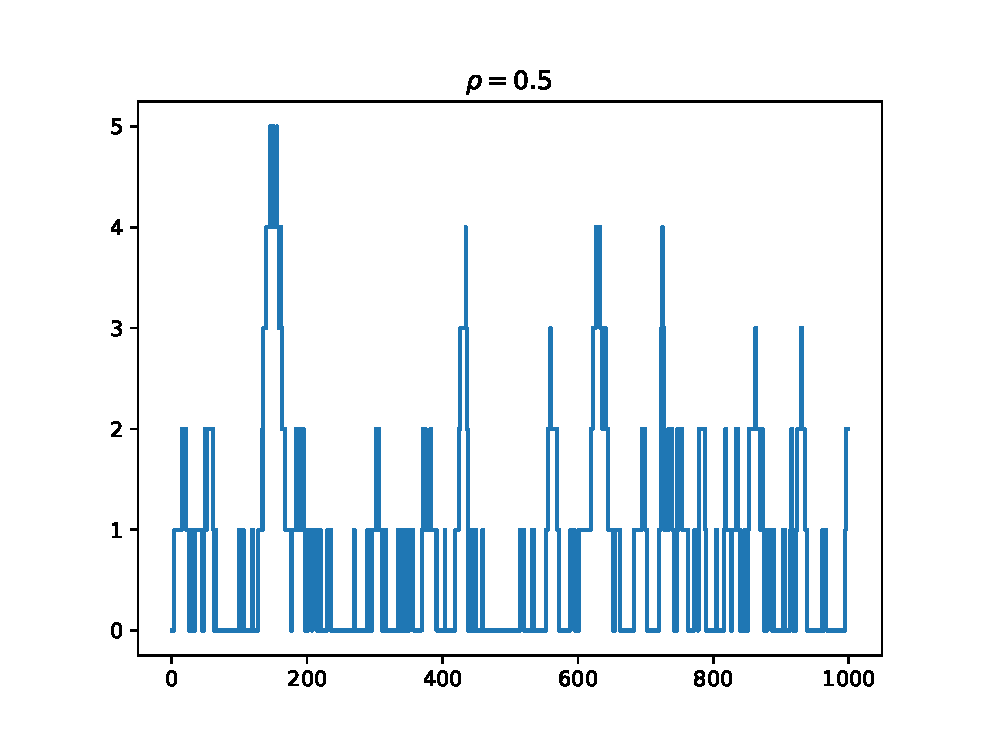
\includegraphics[width=0.8\textwidth]{05.eps}
	\caption{$\mathbf{X}_t$ en fonction du temps pour $\rho = 0.5$.}
\end{figure}
\begin{figure}[H]
	\centering
	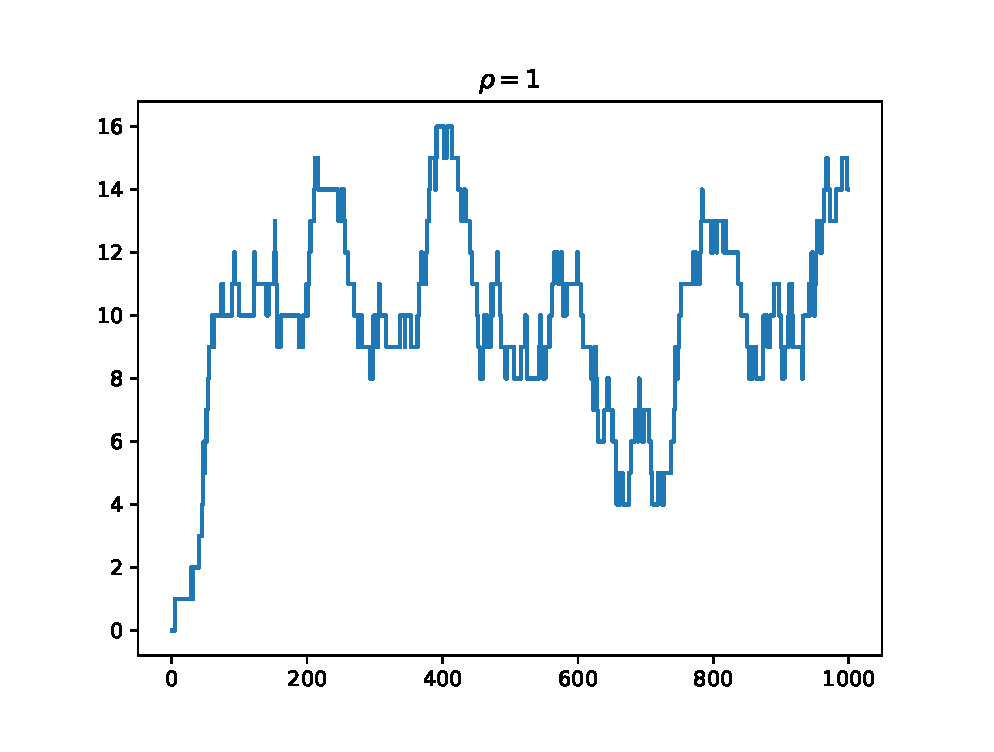
\includegraphics[width=0.8\textwidth]{10.eps}
	\caption{$\mathbf{X}_t$ en fonction du temps pour $\rho = 1$.}
\end{figure}
\begin{figure}[H]
	\centering
	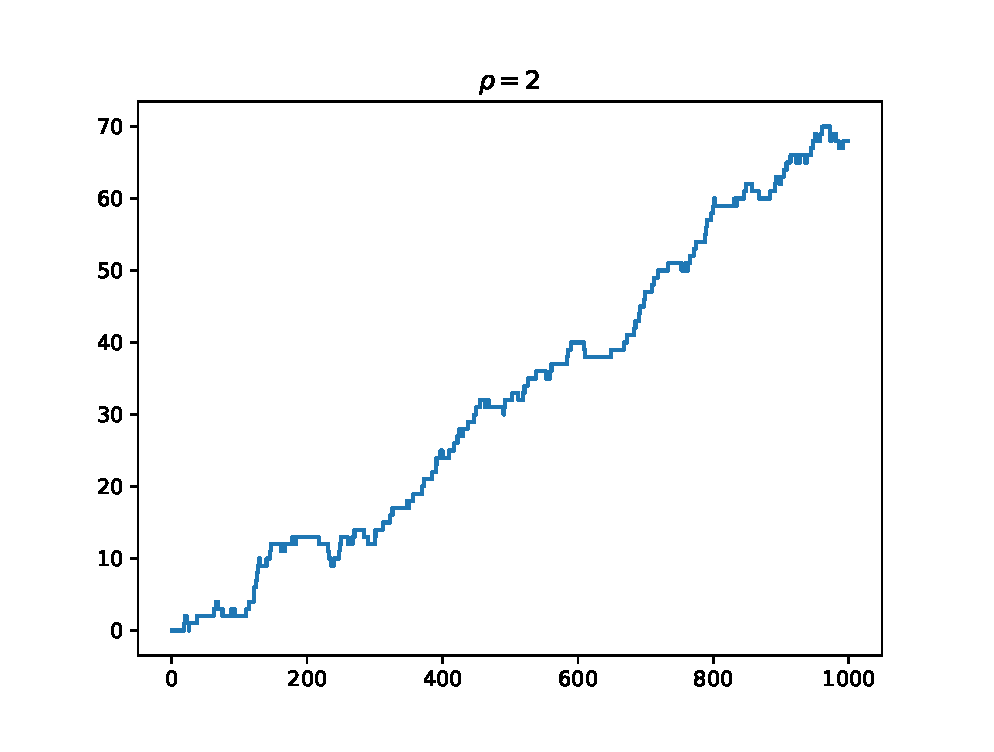
\includegraphics[width=0.8\textwidth]{20.eps}
	\caption{$\mathbf{X}_t$ en fonction du temps pour $\rho = 2$.}
\end{figure}

Comme on peut s'y attendre, lorsque l’espérance des départs est supérieure à l'espérance des arrivées, la quantité de personne en attente stagne dans de petites valeurs. Lorsque $\rho$ vaut 1, le résultat est irrégulier, avec des croissances et décroissances du nombre de personnes arrivant. Le nombre de personne en attente varie plus qu'avant mais reste faible. À l'inverse, lorsque $\rho > 1$, le nombre de personne en attente croit relativement vite.

\paragraph*{Question 2.}

On considère $\rho < 1$. D'après l'énoncé, la moyenne et l'écart type théorique valent en régime stationnaire :

\begin{align*}
\mathbb{E}(X_t) &= \frac{\rho}{1 - \rho} \\
\text{Var}(X_t) &= \frac{\rho}{(1 - \rho)^2}
\end{align*}

Dans notre cas on a $\rho = 0.5$:

\begin{align*}
\mathbb{E}(X_t) &= 1 \\
\text{Var}(X_t) &= 2
\end{align*}

On utilise deux méthodes différentes pour calculer la moyenne et la variance expérimentalement.

Première méthode, on se place en régime stationnaire (donc en $t$ grand) et on simule plusieurs fois la trajectoire. On calcule alors pour un $t$ fixé :

\begin{align*}
\mathbb{E}(X_t) &= 0.924 \\
\text{Var}(X_t) &= 1.861
\end{align*}

Deuxième méthode, on simule une longue trajectoire et par le deuxième point du théorème ergodique, on peut calculer $\pi$ et donc :

\begin{align*}
\mathbb{E}(X_t) &= 0.9909 \\
\text{Var}(X_t) &= 1.9631
\end{align*}

Les erreurs sur le résultat proviennent de la convergence et de la discrétisation en temps.

La seconde méthode semble non seulement plus efficace mais aussi plus rapide. Nous allons donc utiliser celle-ci pour tracer nos courbes d'erreurs.

\begin{figure}[H]
	\centering
	\includegraphics[width=0.95\textwidth]{dt.eps}
	\caption{Convergence pour $\rho = 0.5$ en fonction du pas de discrétisation en temps.}
\end{figure}

% TODO en fonction de rho

\paragraph*{Question 3.}

On trace la distribution de $X_t$ en régime stationnaire. On utilise aussi le théorème ergodique pour calculer $\pi$ de deux façons différentes.

\begin{figure}[H]
	\centering
	\includegraphics[width=0.95\textwidth]{q3.eps}
	\caption{Distribution de $X_t$ en régime stationnaire.}
\end{figure}



\end{document}
